%% Extending Charron (2013) to 2026 -- results deck
%% Compile: pdflatex extension.tex  (run TWICE so the "x/y" page footer resolves
%% \inserttotalframenumber from the .aux)
\documentclass[aspectratio=169,10pt]{beamer}

\usetheme{Madrid}
\usecolortheme{seahorse}
\useinnertheme{rectangles}
\setbeamertemplate{navigation symbols}{}

\usepackage{booktabs}
\usepackage{array}
\usepackage{graphicx}
\usepackage{xcolor}
\usepackage{colortbl}

\definecolor{repcol}{HTML}{1F4E79}     % main (blue)
\definecolor{splitcol}{HTML}{C0504D}   % the 2016-26 split-vote era (red)
\definecolor{jurycol}{HTML}{2E6B34}    % jury-half robustness (green)
\newcommand{\rep}[1]{{\color{repcol}#1}}
\newcommand{\spl}[1]{{\color{splitcol}#1}}
\newcommand{\sg}[1]{\textsuperscript{#1}}
\newcommand{\hd}[1]{\cellcolor{repcol!12}\textbf{#1}}

\title[Charron to 2026]{Extending Charron (2013) to 2026}
\subtitle{Does impartiality still temper friend-voting?}
\author{Eurovision voting-bias project}
\date{\today}

\begin{document}

{\setbeamertemplate{footline}{}
\begin{frame}[plain]
  \titlepage
  \begin{center}\small
  \rep{$\blacksquare$~1975--2026 ESC finals, Charron's own \texttt{eschome} data}\qquad
  \spl{$\blacksquare$~focus: the 2016--2026 split-vote era}
  \end{center}
\end{frame}}

% ---------------------------------------------------------------------------
\begin{frame}{What this tests}
  Charron (2013) found: \textbf{friendship bias shrinks as the voting country's
  institutions become more impartial} (Friend\,$\times$\,Impartiality $<0$), on
  ESC finals \textbf{1975--2012}.  We extend the panel to \textbf{2026} and ask
  whether it still holds --- through the biggest voting-rule change since 1998.
  \vspace{4pt}
  \begin{columns}[T]
    \begin{column}{0.52\textwidth}
      \textbf{Same methodology as the replication}
      \begin{itemize}\small
        \item fn.18 ever-finalist givers; all-voter Quality
        \item cumulative ``2nd-final entry'' cohort
        \item friend groups = Charron's Table 2 (method 1)
        \item estimator = \textbf{R \texttt{AER::tobit}}
      \end{itemize}
    \end{column}
    \begin{column}{0.48\textwidth}
      \textbf{Deliberate deviations (it's an extension)}
      \begin{itemize}\small
        \item impartiality: use \emph{all} available ICRG (keep Balkan voters)
        \item DV: a consistent 0--12 vote; for 2016+ the \textbf{televote half}
          (the 2016+ total is 0--24)
        \item method-2 friends recomputed on the extended data
        \item English/French dropped (no 2024--26 lyrics)
      \end{itemize}
    \end{column}
  \end{columns}
  \vspace{4pt}
  \footnotesize \rep{\textbf{Panel:}} 30{,}599 dyad-years, 1976--2026, 49 countries.
\end{frame}

% ---------------------------------------------------------------------------
\begin{frame}{Four voting-rule eras}
  \centering\small
  \renewcommand{\arraystretch}{1.3}
  \begin{tabular}{@{}l l l l@{}}
    \toprule
    Era & Years & Who decides the points & DV we use\\
    \midrule
    \rep{Jury}     & 1975--1997 & expert juries only            & the 0--12 vote\\
    \rep{Televote} & 1998--2008 & 100\% public televote         & the 0--12 vote\\
    \rep{Hybrid}   & 2009--2015 & 50/50 jury+televote (one 0--12) & the 0--12 vote\\
    \rowcolor{splitcol!12}
    \spl{Split}    & 2016--2026 & jury \emph{and} televote, each 0--12 (total 0--24) & \spl{televote half}\\
    \bottomrule
  \end{tabular}

  \vspace{8pt}
  \footnotesize
  From 2016 the jury and public each award a full 0--12 set, so the raw total is
  0--24 and not comparable to earlier years.  We take the \spl{televote (public)
  half}, the continuation of the public preference measured 1998--2015 --- and check
  the jury half as a robustness test (later slide). \\
  \rep{Era sizes (dyad-years):} jury 8{,}744 \; televote 7{,}020 \; hybrid 6{,}475 \;
  \spl{split 8{,}546}.
\end{frame}

% ---------------------------------------------------------------------------
\begin{frame}{Table 3 (extended) --- the hypothesis still holds, 1975--2026}
  \centering\small
  \renewcommand{\arraystretch}{1.2}
  \begin{tabular}{@{}l c c c c@{}}
    \toprule
    & \hd{All 75--26} & \hd{Jury 75--97} & \hd{Televote 98--26} & \cellcolor{splitcol!15}\spl{\textbf{Split 16--26}}\\
    \midrule
    Quality $C_{jt}$                 & 0.927\sg{***} & 0.880\sg{***} & 0.948\sg{***} & 0.953\sg{***}\\
    Friend Dyad $C_{ijt}$            & 7.24\sg{***}  & 6.16\sg{***}  & 5.30\sg{***}  & 4.30\sg{***}\\
    Impartiality $C_{it}$            & 0.12\ (n.s.)  & $-0.05$\ (n.s.) & 0.07\ (n.s.)  & $-0.25$\ (n.s.)\\
    \rowcolor{yellow!25}
    \textbf{Friend $\times$ Impartiality} & $-5.79$\sg{***} & $-5.54$\sg{***} & $-2.42$\sg{***} & \spl{$-1.41$\ (n.s.)}\\
    \midrule
    $N$                              & 30{,}599 & 8{,}744 & 21{,}855 & 8{,}394\\
    \bottomrule
  \end{tabular}

  \vspace{6pt}
  \footnotesize
  The \colorbox{yellow!25}{Friend\,$\times$\,Impartiality} moderation is negative and
  highly significant across the \emph{whole} 1975--2026 span and through the televote
  era. It \textbf{attenuates} in the recent \spl{split-vote era} ($-1.41$, and n.s.\ in
  this all-controls OLS on just 10 years) --- but stays negative and, in the pooled era
  models (next slides), significant. Quality ($\approx$0.93) and Friend Dyad (large,
  positive) are unchanged.
\end{frame}

% ---------------------------------------------------------------------------
\begin{frame}{The moderation is strongest where juries decide}
  \centering
  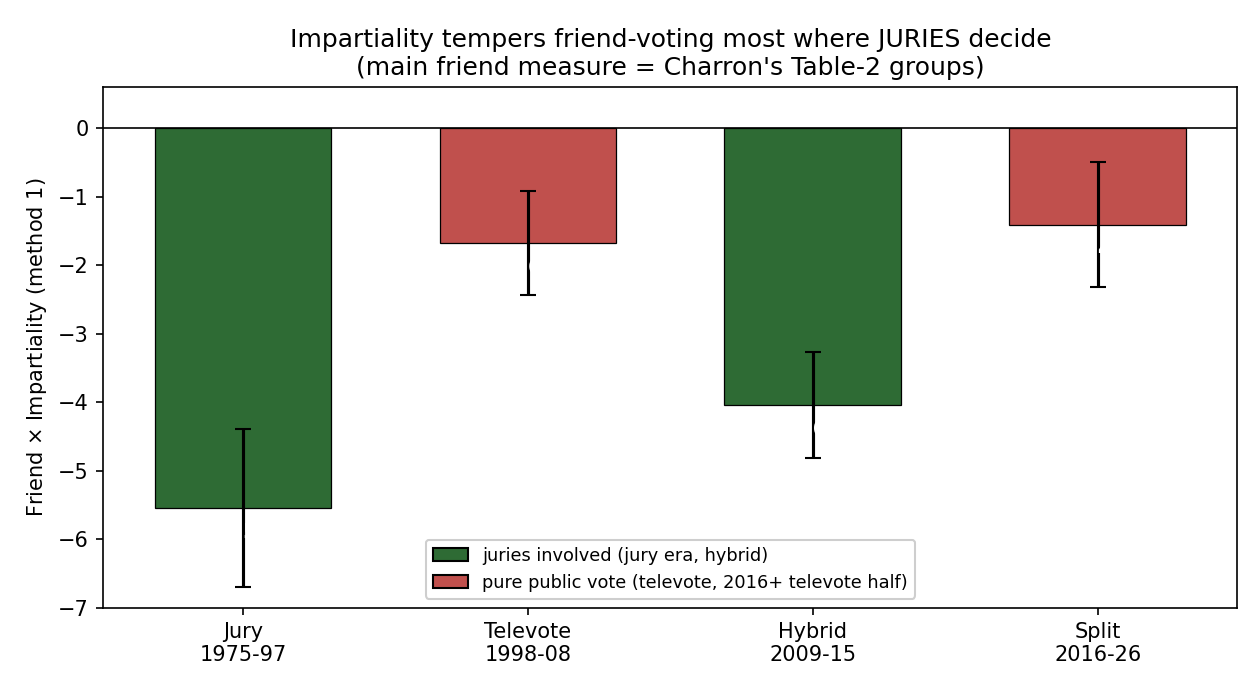
\includegraphics[width=0.68\linewidth]{img/ext_era_interaction.png}

  \vspace{2pt}
  {\footnotesize Friend\,$\times$\,Impartiality by voting-rule era, \textbf{method 1}
  (Charron's Table-2 friend groups --- his \emph{main} measure). Strong where juries
  decide (\color{jurycol}jury era $-5.5$, hybrid $-4.0$\color{black}); weak in the pure
  public vote (\spl{televote 98--08 $-1.7$, 2016+ televote half $-1.4$}).}
\end{frame}

% ---------------------------------------------------------------------------
\begin{frame}{The 2016--2026 split era: the jury advantage has narrowed}
  \centering\small
  \renewcommand{\arraystretch}{1.25}
  \begin{tabular}{@{}l c c@{}}
    \toprule
    \textbf{Friend $\times$ Impartiality}, 2016--26 (\textbf{method 1}) & \spl{Televote half} & \color{jurycol}Jury half\\
    \midrule
    \rowcolor{yellow!25}
    Split era, 2016--2026 & \spl{$-1.41$} (n.s.) & \color{jurycol}$-1.54$\sg{*}\\
    \midrule
    \textit{cf.\ jury era 1975--97} & \multicolumn{2}{c}{\color{jurycol}$-5.54$\sg{***}}\\
    \bottomrule
  \end{tabular}

  \vspace{6pt}
  \footnotesize
  On Charron's \textbf{main} friend measure, in the newest era the jury and public halves
  are \colorbox{yellow!25}{statistically indistinguishable} ($-1.54$ vs $-1.41$, both
  weak) --- the strong discipline juries once provided ($-5.54$ in 1975--97) has
  \textbf{faded even on the jury side}. So the ``expert-judgment'' story is a statement
  about the \emph{whole record} (next slide), not the 2016+ split specifically.
  \footnotesize (The pairwise robustness measure does still show a jury-half gap,
  $-3.78$ vs $-2.33$, but the main measure does not.)
\end{frame}

% ---------------------------------------------------------------------------
\begin{frame}{Jury vs public channel --- pooled across \emph{all} years}
  \begin{columns}[T]
    \begin{column}{0.60\textwidth}
      \centering
      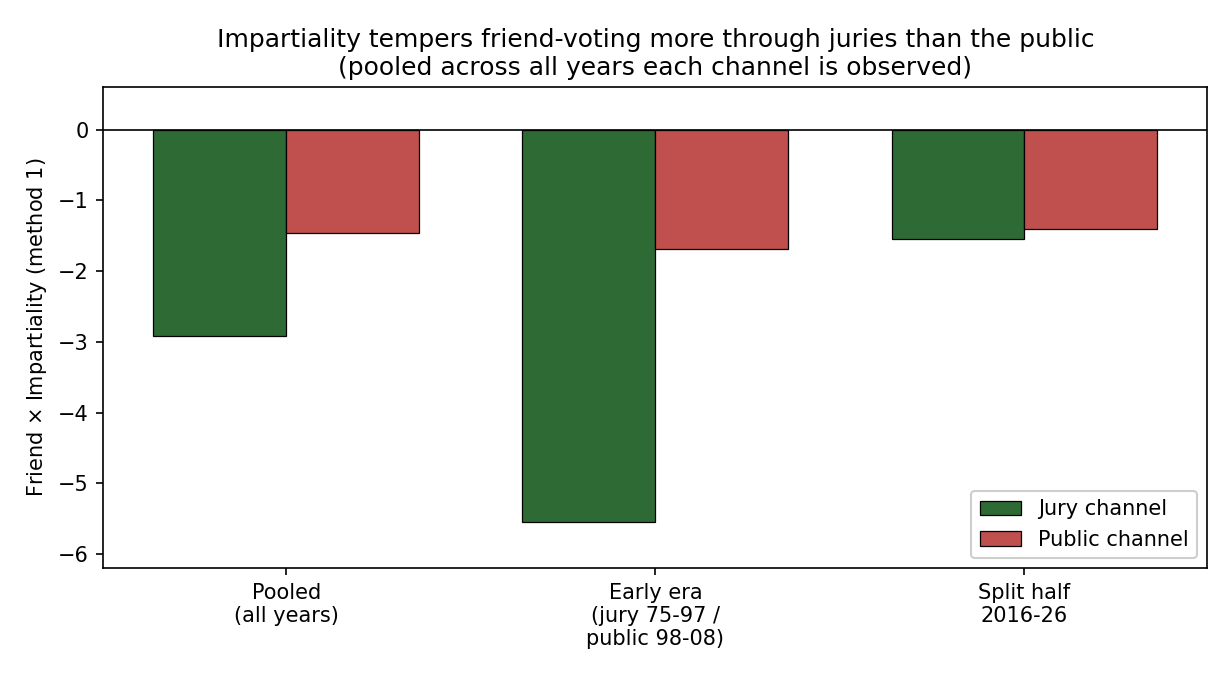
\includegraphics[width=\linewidth]{img/fig_channels.png}
    \end{column}
    \begin{column}{0.40\textwidth}\small
      Two panels, each pooling every year the channel is cleanly observed:
      \begin{itemize}\footnotesize
        \item \textbf{\color{jurycol}Jury} = 1975--97 (juries) + 2016--26 jury half
        \item \spl{\textbf{Public}} = 1998--08 (televote) + 2016--26 televote half
      \end{itemize}
      \vspace{2pt}
      Friend\,$\times$\,Impartiality is \textbf{$\approx$2$\times$ stronger through
      juries} (\color{jurycol}$-2.92$\color{black}) than the public
      (\spl{$-1.46$}). It is the early expert-jury era that carries it; in the recent
      \spl{split} era both halves are weak. \\[3pt]
      \footnotesize (2009--15 hybrid is a single combined score, so it can't enter
      either pure channel.)
    \end{column}
  \end{columns}
  \vspace{2pt}
  {\footnotesize Charron's mechanism on the full record: impartiality disciplines
  friend-voting mainly through \emph{expert} judgment.}
\end{frame}

% ---------------------------------------------------------------------------
\begin{frame}{The Rest-of-World vote --- an ``impartial voter'' benchmark}
  \begin{columns}[T]
    \begin{column}{0.55\textwidth}
      \centering
      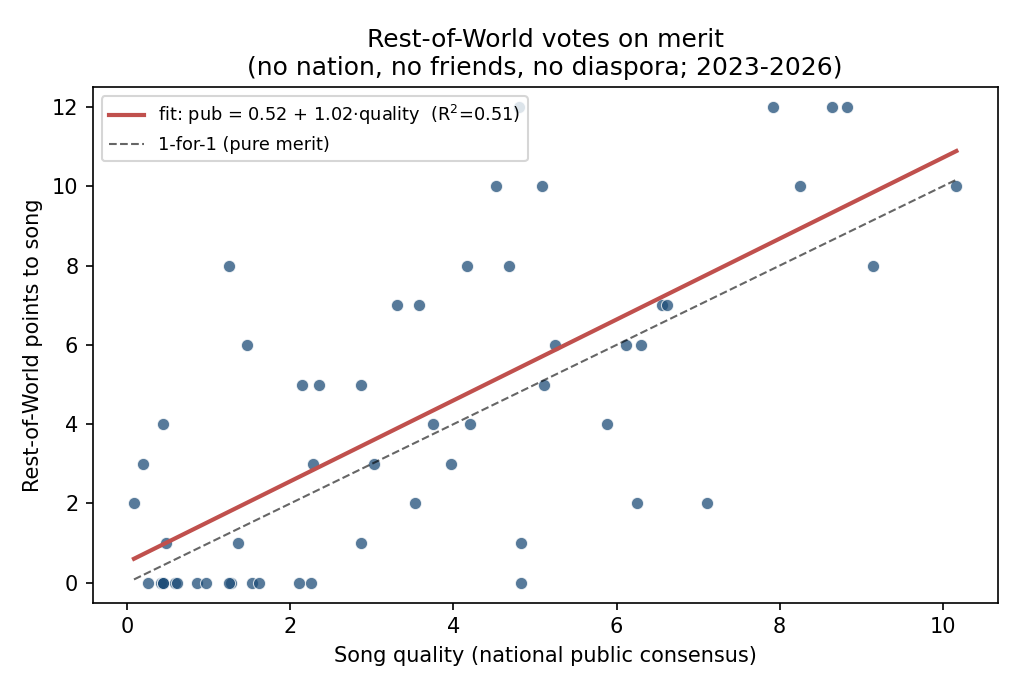
\includegraphics[width=\linewidth]{img/fig_restofworld.png}
    \end{column}
    \begin{column}{0.45\textwidth}\small
      Since 2023 an aggregate \textbf{global online televote} (``Rest of the World'')
      awards a normal 0--12 set --- but has \textbf{no nation, no friends, no
      diaspora}. A natural benchmark:
      \begin{itemize}\footnotesize
        \item rewards quality \textbf{$\approx$1-for-1} (slope \rep{1.02}, R$^2$ 0.51)
          --- \emph{more} meritocratic than national voters (0.92)
        \item \textbf{no friend-bloc premium} ($-0.16$, n.s.)
        \item lacks the diaspora bias national electorates show
          (national $+0.79$\sg{***} per rank; RoW $=0$)
      \end{itemize}
      \vspace{2pt}
      So the global audience votes on \textbf{merit} --- confirming the model's
      friend/diaspora effects are about \emph{national} ties, not song popularity.
      \footnotesize (Only 56 RoW dyads, 2023--26; the quality result is the robust one.)
    \end{column}
  \end{columns}
\end{frame}

% ---------------------------------------------------------------------------
\begin{frame}{What else carries through to 2026}
  \centering\small
  \renewcommand{\arraystretch}{1.25}
  \begin{tabular}{@{}l c l@{}}
    \toprule
    Effect & Extended estimate & Reading\\
    \midrule
    Quality $C_{jt}$        & 0.93--0.95\sg{***} & song quality still drives $\approx$1-for-1\\
    Friend Dyad $C_{ijt}$   & +4 to +7\sg{***}   & friends still bias, every era\\
    \rowcolor{yellow!25}
    Diaspora $C_{ji}$       & +0.24 to +0.56\sg{***} & diaspora still rewards the homeland\\
    Contiguity $C_{ij}$     & +0.9 to +1.4\sg{***} & neighbours still trade votes\\
    Language $C_{ij}$       & +0.3 to +0.6\sg{***} & shared language still matters\\
    Impartiality (alone)    & $\approx$0\ (n.s.)   & no effect among non-friends (as in Charron)\\
    \bottomrule
  \end{tabular}

  \vspace{6pt}
  \footnotesize
  Every structural feature of Charron's model survives the 14-year extension and the
  2016 rule change. The \colorbox{yellow!25}{Diaspora} effect --- his ``pioneering''
  control --- remains positive and significant right through 2026.
\end{frame}

% ---------------------------------------------------------------------------
\begin{frame}{Takeaways}
  \begin{enumerate}
    \item \textbf{The finding extends.} Across 1975--2026, impartial countries temper
      their friend-voting bias (Friend\,$\times$\,Impartiality $<0$) --- negative and
      significant pooled and in every voting-rule era.
    \item \textbf{It attenuates in the mass-public-vote eras}, not reverses: weakest
      under 100\% televoting (98--08) and in the \spl{2016--2026 split era}.
    \item \textbf{The mechanism is expert judgment.} Pooled across all years, the
      moderation is $\approx$2$\times$ stronger through the \color{jurycol}jury channel
      \color{black}($-2.92$) than the \spl{public channel} ($-1.46$) --- impartiality
      disciplines friend-voting mainly via expert juries.
    \item \textbf{The Rest-of-World vote is the impartial benchmark.} With no nation or
      diaspora, the global online audience rewards quality $\approx$1-for-1 and shows
      none of the diaspora bias ($+0.79$\sg{***}) of national electorates.
    \item \textbf{The rest of the model is stable}: Quality $\approx$0.93, Friend Dyad
      large \& positive, Diaspora/Contiguity/Language all significant through 2026.
  \end{enumerate}
  \vspace{4pt}
  \footnotesize\rep{Estimated in R (\texttt{AER::tobit}) on the same Python-built panel
  as the replication; Charron's own \texttt{eschome} data, through Eurovision 2026.}
\end{frame}

\end{document}
